\chapter{Introduction}
\label{ch:intro}
Plasma medicine is an emerging field that is broadening its applications from uses on medical equipments (sterilization, decontamination) to uses on living tissues \cite{plmed_review}. One of the reserch groups working in Consorzio RFX laboratories, in Padova, developed a source for the production of Cold Atmospheric Plasma (CAP) to be used for medical treatment on biological tissues: Plasma Coagulation Controller (PCC) \cite{DeMasi_2018}. The source is a Dielctric Barrier Discharge reactor, where a dielectric is used to produce plasma with low charge density. It is developed to promote non thermal blood coagulation, i.e. acceleration of blood clot formation thanks to plasma direct application.

CAPs are of particular interest in plasma medicine for two characteristics:
\begin{itemize}
 \item \textbf{Cold plasma} : given non thermal equilibrium and ion low temperature, this plasma can be applied on surfaces without a dangerous increase in target temperature. In plasma medicine CAPs allow treatment on living tissues, where target temperature must be kept below a safe value.
 \item \textbf{Reactive Species} : When a gas is ionized at atmospheric pressure, the produced plasma is mixed with the surroundig air molecules. The peculiarity of a plasma in air is the presence of reactive species, ions, produced by ionization and recombination of nitrogen, oxygen, water and other atoms or molecules. There are several biological processes where activation and reactions speed is thought to be related to concentration of Reactive Oxydant Species (ROS) and Reactive Nitrogen Species (RNS) \cite{doi:10.1152/ajplung.2000.279.6.L1005}, \cite{doi:10.1152/ajpcell.00366.2006}. 
\end{itemize}

In this chapter there is the presentation of some results obtained with PCC and a general description of the production of CAP, describing the sources developed at Consorzio RFX.

\section{Plasma medicine}
The most studied therapeutic effects of plasma application are:
\begin{itemize}
 \item sterilization and decontamination \cite{Martines_2009}, \cite{Stoffels_2007};
 \item blood coagulation \cite{Fridman2006};
 \item wound disinfection and healing \cite{Haertel2014};
 \item cancer cell treatment \cite{Yan2016}.
\end{itemize}
How plasma interacts with living tissues and produces those effects is not fully understood. Reactive species, along with UV radiation and electromagnetic field, are considered fundamental partecipants of the mechanism.

Previous works studied PCC induced bactericidal effects and non thermal blood coagulation; in the following their results will be described briefly.

\paragraph{Bactericidal effects}
There are numerous studies on the effects of CAPs on bacteria \cite{1167632}, \cite{1673530}, however mechanisms leading to inactivation of bacteria are not fully understood. It is tought that plasma application has an effect when reactive species, UV photons and charged particles comes into direct contact with cell's membrane and structures \cite{plmed_review}.

In figure \ref{fig:bact} is presented the reduction of bacteria vitality due to application of plasma produced with our sources. From the figure it's possible to see results of the experiment on three different bacteria species, for an RF source and for the DBD source, PCC, with three different experimental setups. PCC seems to have a faster effect on the reduction of bacteria, for all analyzed species. 
\begin{figure}
 \centering
 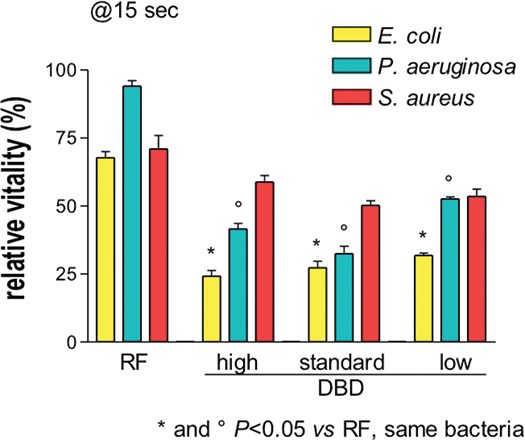
\includegraphics[width=0.5\textwidth]{Images/Intro/bacteria2.png}
 \caption{Relative vitality on different bacteria colonies after plasma treatment of \SI{15}{\second} with different sources. On the left there is treatment with an RF plasma source; on the right there is treatment with the DBD plasma source studied in this work, PCC, for three different combinations of parameters for the discharge (low, standard and high).}
 \label{fig:bact}
\end{figure}


\paragraph{Blood coagulation}
Cauterization devices that produce quasi-thermal blood coagulation with high-temperature plasma have been used for a long time in wound treatment and surgery. Only recently studies shown that with cold plasma application is possible to induce natural blood coagulation, without temperature increase \cite{Fridman2006}, \cite{4343167}.
Treatments with CAPs activate the coagulation cascade shown in figure \ref{fig:coag}, a chain of reactions that involves many tissue factors and proteins. The exact mechanisms that accelerates clot formation have to be understood yet, as of today studies show that plasma induces the production of fibrin that catalyses blood coagulation factors \cite{plmed_review}.
\begin{figure}
 \centering
 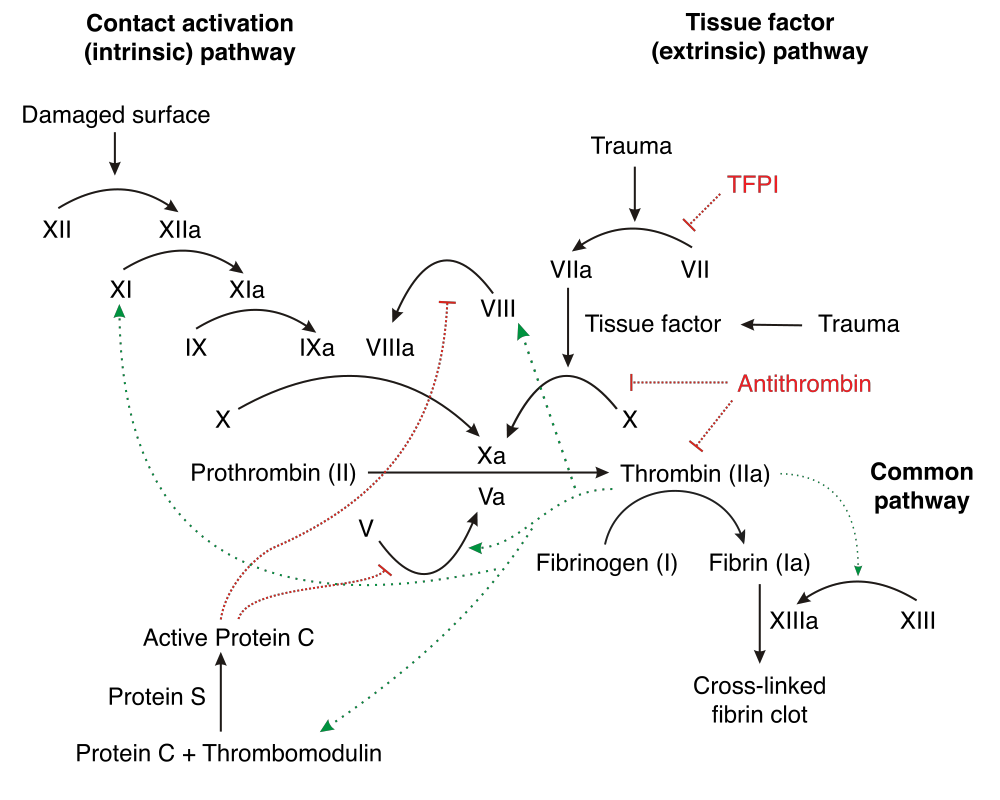
\includegraphics[width=0.8\textwidth]{Images/Intro/coag_map.png}
 \caption{Reaction chain that leads to blood coagulation. The analysis of blood samples treated with plasma, allows to find where and how plasma intervenes in this scheme.}
 \label{fig:coag}
\end{figure}


Treatment with PCC is done applying plasma on blood samples, as shown in figure \ref{fig:plasmaapp} (a). The study involves the use of different plasma application times and different discharge parameters. The effect of plasma application is evaluated from samples as those in figure \ref{fig:plasmaapp} (b), where the blood is removed and the area of the remaining coagulated blood is measured, leading to results in figure \ref{fig:plasmaapp} (c). Results show always an increase on blood coagulation when treated with plasma. 
\begin{figure}
 \centering
 \subfloat[Picture of plasma application.] {
    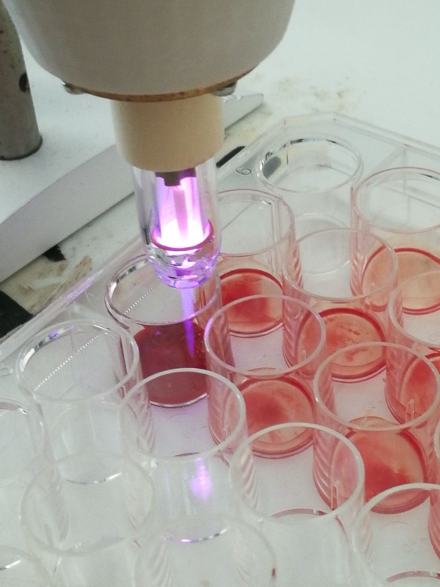
\includegraphics[width=0.4\textwidth]{Images/Intro/source_application.png}
 }
 \hfill
 \subfloat[Coagulated blood samples.]{
    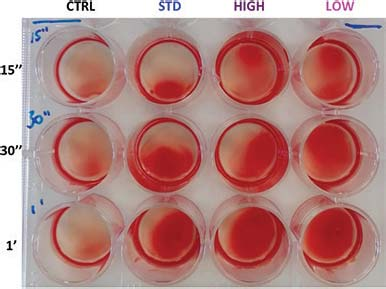
\includegraphics[width=0.5\textwidth]{Images/Intro/blood_sample.png}
 }
 \vspace{1cm}
 \subfloat[Coagulated blood area.]{
    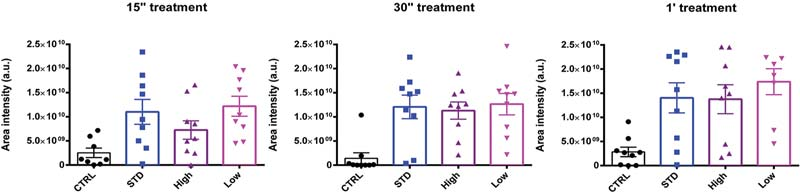
\includegraphics[width=\textwidth]{Images/Intro/coag_histo.png}
 }
 \caption{Pictures and results of the blood coagulation study with PCC. Blood samples are treated with three different parameters of the DBD discharge, for three different application times. In (c) is possible to see the increse of coagulated blood area for samples treated by plasma, if compared to the control sample.}
 \label{fig:plasmaapp}
\end{figure}


\begin{comment}
\paragraph{ROS and RNOS presence}

\begin{figure}
 \centering
 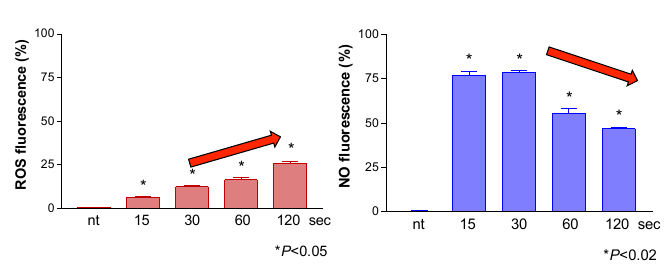
\includegraphics[width=0.4\textwidth]{Images/Intro/ROS.png}
 \caption{ROS and NO fluorescence }
 \label{fig:ROS}
\end{figure}
\end{comment}


\section{Cold Atmospheric Plasma}
In a CAP thermodynamical equilibrium is not reached. Electron energy is usually much higher than ion energy \cite{VONENGEL196599}. In those conditions plasma dynamics can be described as the collective motion of two interpenetrating fluids, where the thermal motion of ions can be ignored \cite{goossens2012introduction}.
There are several studies on CAP plasma characteristics \cite{Zhu_2009}, \cite{Ohyama_2009}, \cite{Amorim_2015} typical values are electron temperatures between $T_e = 1 - \SI{10}{\electronvolt}$ and electron densities between $n_e = \num{e17} - \SI{e22}{\meter^{-3}}$ , inside the box outlined in figure \ref{fig:plasmaclass}. 
\begin{figure}
 \centering
 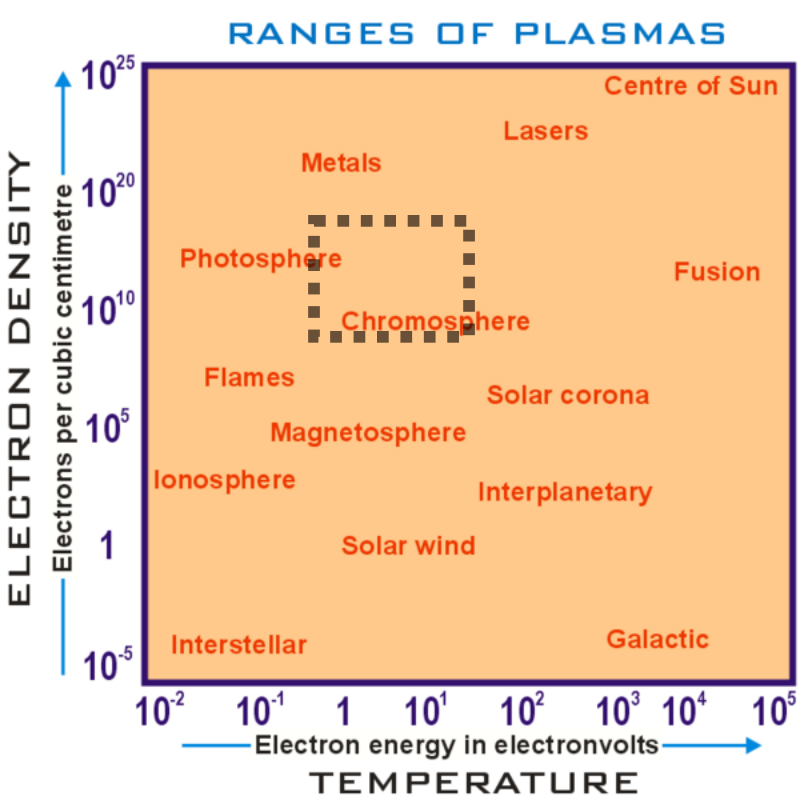
\includegraphics[width=0.5\textwidth]{Images/Intro/Plasma_classification2.png}
 \caption{Plasma classification in function of electron density and electron temperature. Inside the square there are typical parameters for CAPs.}
 \label{fig:plasmaclass}
\end{figure}


\subsection{Plasma generation}
Electron density in CAPs is much smaller than the neutral density of an ideal gas $n_{n} = \SI{2.50e25}{\meter^{-3}}$. However it is higher than the density of free electrons naturally present in air at atmospheric pressure. Radioactive substances and cosmic rays generates electron-ion pairs with a total ionization rate of $\SI{e7}{\meter^{-3}\second^{-1}}$ \cite{book:1593058}.

The application of a steady electric field to a gas accelerate free electrons that collide with atoms and molecules resulting in excitation or ionization reactions. If the electric field has enough intensity it extract electrons from atoms and molecules ionizing them. Those reactions form ion-electron pairs that are accelerated producing other pairs, inducing chain reactions that could sustain plasma discharge. If and how this process starts is influenced by:
\begin{itemize}
 \item gas species, by their ionization potential and cross section for different reactions
 \item characteristics lenght of the system, that influences charged particle's acceleration
 \item gas pressure, that is proportional to reaction rates
\end{itemize}
%The breakdown conditions are defined by the well known Paschen curves, where the voltage breakdown potential is studyed for different values of the product of electrodes distance and gas pressure, related respectively to electron acceleration and collisions frequency.

Generally electrons acquire more energy from the electric field due to the lower mass and higher mobility, so electronic temperature increases more rapidly then ion temperature. If we apply a steady DC electric fields, electrons and ions reach thermal equilibrium trough collisions, generating thermal plasma at high temperatures. To avoid thermalization and produce cold plasma at high densities is possible to give energy selectively to electrons with AC electric fields at high frequency \cite{BARDOS20106705}.


Two examples of sources that produce plasma for medical application are the ones built at RFX: the RF source based on a radio transmitter (\cite{Martines_2009}) and the DBD source, studied in this work (\cite{DeMasi_2018}).

\paragraph{RF source}
The RF source developed in RFX works applying an AC electric field between two electrodes. It is composed by two coaxial tubes as shown in figure \ref{fig:RF}: the internal one is connected to a radio transmitter in series with a matching network and with an electrode formed by a wire grid; the external one ends with a second electrode fixed at ground potential. The radio transmitter works with fixed power (\SI{5}{\watt}) and is set to a specific frequency that is the resonance frequency for the LC series circuit formed by the induttance in the matching network and the parasitic capacitance of the device. When neutral gas flows inside the inner tube, the electric field between the electrodes ionizes it, producing cold plasma in air. The source is built with an induttance of \SI{100}{\micro\henry}, capacitance is estimated as \SI{10}{\pico\farad}, resulting in a resonance for a frequency around \SI{4.8}{\mega\hertz}, reaching voltage peak to peak values up to \SI{900}{\volt} on the electrode. By setting an appropriate gas flow, the discharge starts more easily and to reach lower peak voltage values.
This source produces plasma directly in air, so it ionizes a mixture of neutral gas and air, giving birth to plasma rich in reactive species coming from oxygen and nitrogen molecules. The presence of reactive species allows to use this source for non-thermal sterilization of living tissues: plasma produced by it has bactericidal effects and does not damage human cells (\cite{doi:10.1002/ppap.200700154}).
\begin{figure}
 \centering
 \subfloat[Source scheme.]{
    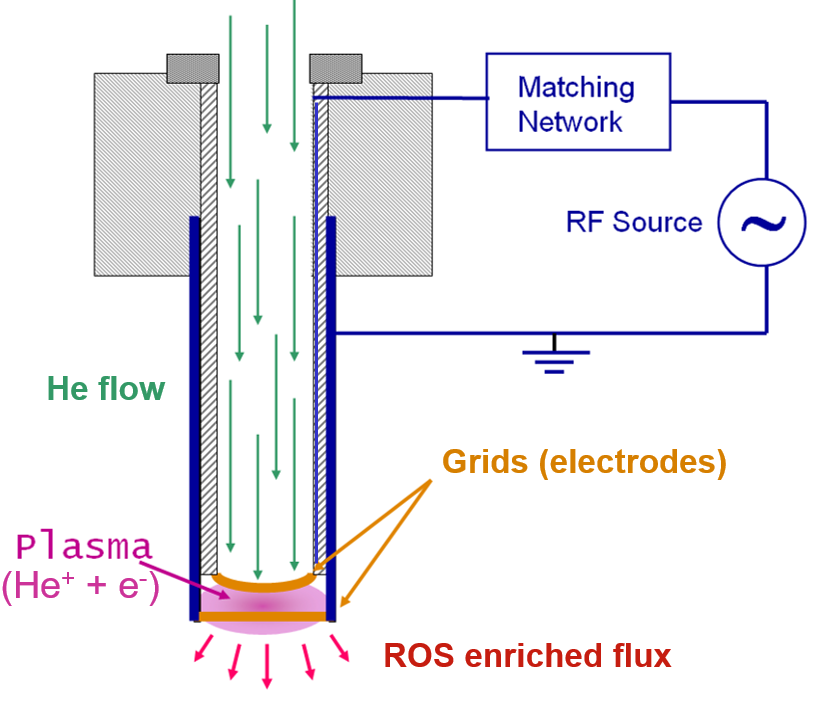
\includegraphics[width=0.4\textwidth]{Images/Intro/RF.png}
 }
 \hfill
 \subfloat[Picture of produced plasma.]{
    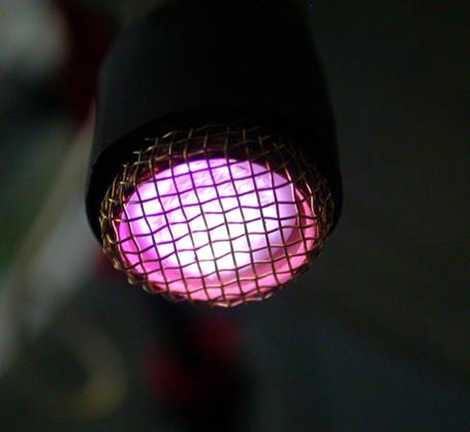
\includegraphics[width=0.4\textwidth]{Images/Intro/RF_plasma.png}
 }
 \caption{Plasma RF source developed in RFX.}
 \label{fig:RF}
\end{figure}


\paragraph{DBD source}
The source developed in this work is based on the Dielectric Barrier Discharge (DBD): it applies an electric field on the gas with one electrode or a pair of electrodes, where a dielectric covers at least one of them, as in figure \ref{fig:DBDex}.
The dielectric works as an insulator and does not allow DC current to flow in the gap, so gas between the electrodes can be ionized without large current densities flowing trough the resulting plasma (\cite{Kogelschatz2003}). The discharge can be modelized as in the circuit in figure \ref{fig:DBDex} (b) (\cite{DBDcircuit}), $C_1$ is capacitance of dielectric, $C_2$ of air and $R_p$ and $C_p$ are plasma resistance and capacitance (in other studies it is possible to find more refined models \cite{doi:10.1063/1.4986023}). Typical values for discharge parameters are AC voltage frequency or pulse rates $f \ge \SI{1}{\kilo\hertz}$, voltage peak values from $V_{p} = 1 - \SI{20}{\kilo\volt}$, and current peak intensities on a conductive target $I < \SI{100}{\milli\ampere}$.
\begin{figure}
 \centering
 \subfloat[DBD scheme with two electrodes.]{
    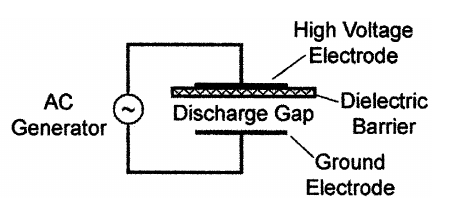
\includegraphics[width=0.48\textwidth]{Images/Intro/DBD_es1.png}
 }
 \hfill
 \subfloat[DBD circuit diagram.]{
    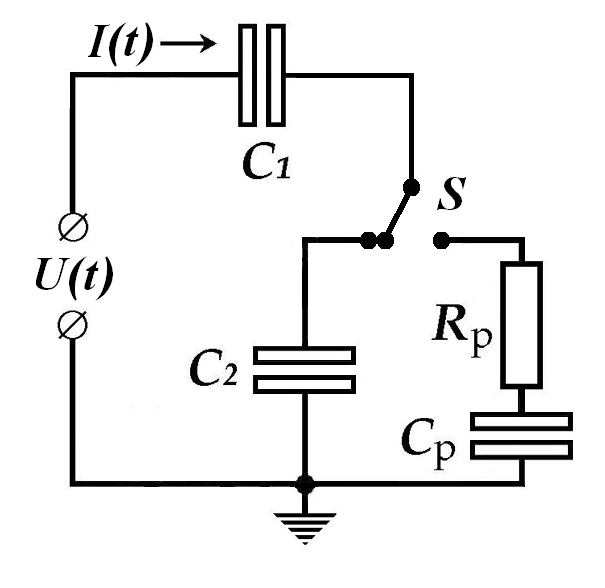
\includegraphics[width=0.4\textwidth]{Images/Intro/Fig1DBD.png}
 }
 \caption{Representation of the concept behind DBD plasma production: on the left  an experimental setup composed by two electrodes, one dielectric and a voltage AC generator; on the right a circuit diagram of the setup for DBD discharge. In the circuit, $C_1$ is the dielectric capacitance, $C_2$ the air capacitance, $C_p$ and $R_p$ are plasma capacitance and resistance.}
 \label{fig:DBDex}
\end{figure}

DBD plasma reactors changed in the last decades following the development of pulse power technology: from the classic sinusoidal voltage now is common to apply pulsed voltage. Plasma generated with sub-microseconds voltage pulses allows to avoid local discharges overheat and increases discharge production of reactive species inside the plasma (\cite{SHAO2009215}). Those progresses in DBD plasma technology led to the development of sources for biomedical plasma applications. Those plasma sources, including PCC, have to produce plasma rich in reactive species, while meeting stringent requirements such as low temperature (at or near room temperature), no risk of arcing, operation at atmospheric pressure, preferably hand-held operation, low concentration of ozone generation, etc.

The design used in many works is in figure \ref{fig:DBDmed} (\cite{Stoffels_2006}, \cite{doi:10.1063/1.2045549}): a cylindrical electrode is covered in dielectric material and inserted in a tube with neutral gas flowing in it. The gas, typically helium or argon, allows to start plasma discharge, then plasma is expelled in air where it produces reactive species needed for medical treatment. PCC developed and studied in this thesis will be described in details in chapter \ref{ch:electric}, along with its electrical characterization.
\begin{figure}
 \centering
 \subfloat[\emph{Plasma pencil} \cite{Stoffels_2006}.]{
    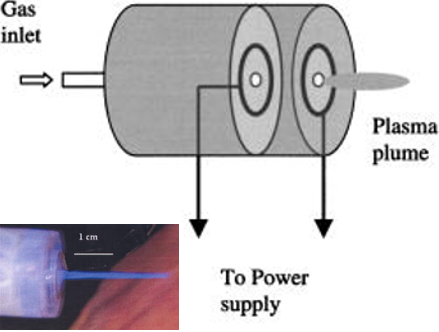
\includegraphics[width=0.4\textwidth]{Images/Intro/DBDmed5.png}
 }
 \hfill
 \subfloat[\emph{Plasma needle} \cite{doi:10.1063/1.2045549}.]{
    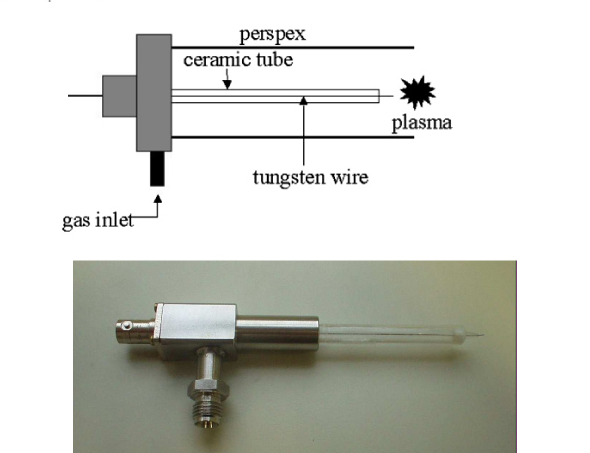
\includegraphics[width=0.4\textwidth]{Images/Intro/DBDmed4.png}
 }
 \caption{Two example of DBD plasma sources for medical applications. In both sources we have one electrode that applies an electric field to neutral gas, ionizing it. Plasma is then expelled in air at atmospheric pressure.}
 \label{fig:DBDmed}
\end{figure}


An intersting phenomenon in sources with this design is plasma formation and propagation. High speed camera measuraments of the process show that plasma is not produced in a uniform steady column, but every pulse of the electric field gives start to localized plasma emission. Once produced, the ionization wave moves from the electrode and propagates in air, with velocities from \num{10} to over \SI{150}{\kilo\meter/\second}. Those localized plasma emissions are called ``bullet'' and only recently is possible to find models that describe them \cite{Lu2016DynamicsOA}.
In this thesis this phenomenon is observed and sudied in details in chapter \ref{ch:shape}, with different voltage pulse parameters, target position and gas composition.


As said before, the purpose of non thermal plasma application for medical uses is the deposition of reactive species on biological tissues. The presence and chracteristics of reactive species can be studied by emission spectroscopy, with intensity and temperature estimation. Chapter \ref{ch:spectrometry} is dedicated to the study of plasma radiation emission around visible wavelengths.


The other fundamental feature of plasma produced by our source is that can be applied on human body without danger. Temperature measurements on the target of plasma application can lead to an estimation of plasma power deposition. In chapter \ref{ch:temperature} are presented thermocamera mesurements and power estimation.
